\documentclass{article}

\usepackage{ragged2e}
\usepackage{graphicx}
\usepackage{caption}
\usepackage{tikz}
\usetikzlibrary{automata, positioning, arrows}

\captionsetup{font=footnotesize}

\begin{document}
\title{Prova Finale di Reti Logiche}
\author{Andrea Sanvito}
\date{15 Maggio 2024}
\maketitle
\noindent
\begin{center}
\begin{tabular}{l r}
Matricola: & 983819 \\
Codice Persona: & 10814394 \\
\end{tabular}
\end{center}
\vspace*{3cm}
\section{Requisiti del Progetto}
\subsection{Overview}
Il progetto riguarda l'implementazione in VHDL di un modulo in grado di modificare una memoria RAM, seguendo determinate specifiche.

In particolare, viene dato in input al modulo un indirizzo da 16 bit della memoria addr e un valore intero k da 10 bit.
Compito del modulo è quello di:
\begin{itemize}
    \item accedere alla RAM all'indirizzo fornito in input;
    \item considerare la memoria come una sequenza di "coppie" di numeri, dove il primo rappresenta un dato, e il secondo un
    valore di credibilità del dato stesso.
    \item scorrere le k coppie in memoria una ad una, e ad ogni passo:
    \begin{itemize}
        \item se il dato è specificato (ossia diverso da zero), lo si mantiene in memoria e si imposta il valore di credibilità seguente al massimo;
        \item altrimenti, si aggiorna il dato in memoria con l'ultimo dato valido letto, e si decrementa il valore di credibilità;
    \end{itemize}
\end{itemize}

L'implementazione deve essere completamente sincrona con un segnale di Clock fornito esternamente, eccetto per il segnale di Reset, che è invece asincrono.
E' riportato di seguito un esempio.

\subsection{Esempio}
Consideriamo l'indirizzo di memoria iniziale addr pari a 128, mentre k pari a 16.

\begin{figure}[h]
    \centering
    \includegraphics[width=1\textwidth]{example.png}
    \caption[short]{memoria RAM prima e dopo le operazioni svolte dal modulo}
\end{figure}

Il nostro modulo accede alla RAM all'indirizzo specificato e legge il dato: essendo questo diverso da zero, lo salva come "ultimo valore valido" e porta il valore di credibilità al massimo (da specifica, il massimo equivale a 31) e lo scrive nella cella seguente.\\
La cella successiva a quella appena scritta contiene uno zero, ossia un valore non specificato: il modulo lo sostituisce inserendo l'ultimo valore valido, e decrementa la credibilità, scrivendola nella cella successiva. 
Così, fino alla cella all'indirizzo 134, dove troviamo un dato diverso da zero: il modulo procede a sostituire l'ultimo valore valido letto, e a riportare la credibilità a 31, scrivendola nella cella successiva.
Queste azioni vengono ripetute fino a quando k, il quale viene decrementato ogni volta che si legge un dato, arriva a zero.

\subsection{Ipotesi Progettuali}
Il progetto è stato svolto con determinate ipotesi:
\begin{itemize}
    \item l'indirizzo addr deve essere valido, ossia non deve essere oltre l'ultimo indirizzo di memoria della RAM;
    \item la somma tra addr e k deve essere valida, ossia non deve andare oltre l'indirizzo finale della RAM; 
\end{itemize}
Il comportamento del modulo implementato non è specificato per i casi sopra elencati.

\newpage
\section{Architettura}
\subsection{Overview}
L'implementazione è stata ottenuta attraverso un singolo modulo, una FSM, con due processi.
Essa comunica con la memoria, esegue computazione, e asserisce gli output.

\begin{figure}[ht]
    \centering
    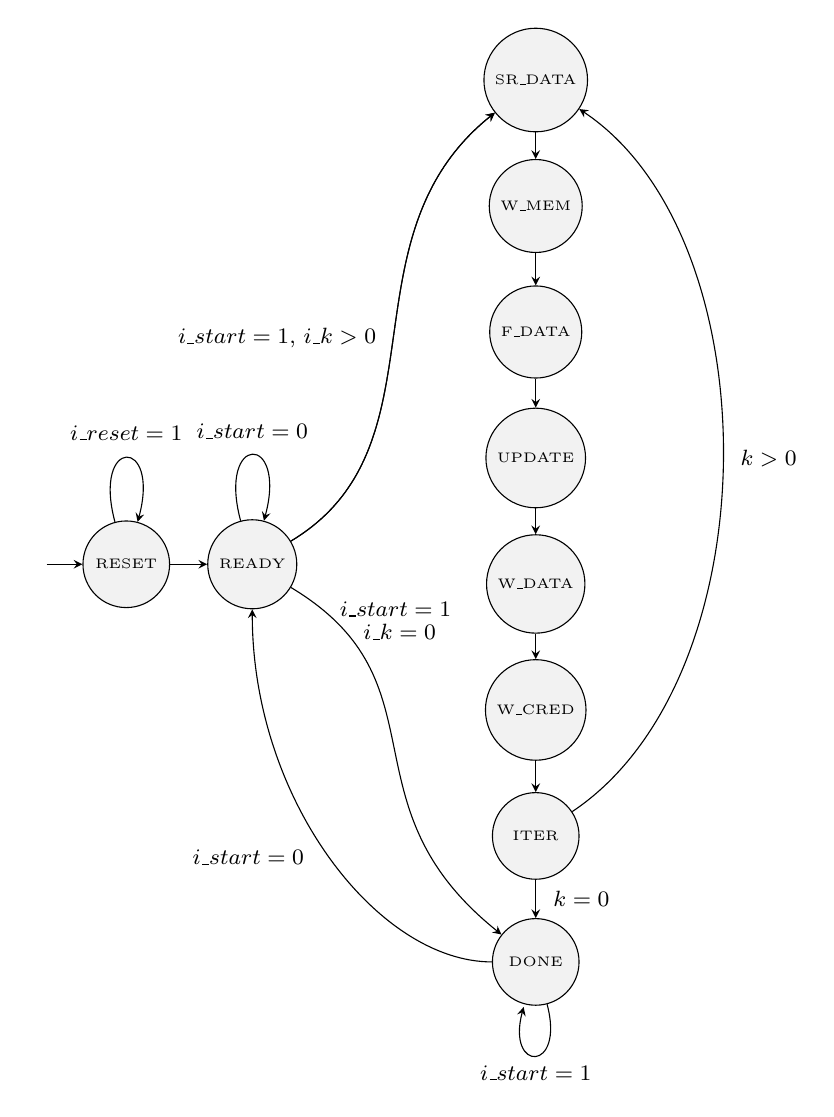
\begin{tikzpicture}[]
        \tikzset{
            ->,  % makes the edges directed
            >=stealth, % makes the arrow heads bold
            node distance=1.6cm, % specifies the minimum distance between two nodes. Change if n
            every state/.style={fill=gray!10, minimum size = 1.1cm}, % sets the properties for each ’state’ n
            initial text=$ $, % sets the text that appears on the start arrow
            }

        % nodes
        \node[state, initial] (reset_state) {\tiny RESET};
        \node[state, right of=reset_state] (ready_state) {\tiny READY};
        \node[state, right of=ready_state, xshift=2cm, yshift=1.35cm] (update_state) {\tiny UPDATE};
        \node[state, above of=update_state] (fetch_data_state) {\tiny F\_DATA};
        \node[state, above of=fetch_data_state] (wait_mem_state) {\tiny W\_MEM};
        \node[state, above of=wait_mem_state] (set_read_data_state) {\tiny SR\_DATA};
        \node[state, below of=update_state] (write_data_state) {\tiny W\_DATA};
        \node[state, below of=write_data_state] (write_cred_state) {\tiny W\_CRED};
        \node[state, below of=write_cred_state] (iterate_state) {\tiny ITER};
        \node[state, below of=iterate_state] (done_state) {\tiny DONE};
    
        % reset state paths
        \path (reset_state) edge (ready_state);
        \path (reset_state) edge [loop above, looseness=10] node [yshift=0.1cm] {\footnotesize \(i\_reset = 1\)} (reset_state);
        
        % ready state paths
        \draw (ready_state) .. controls ++(2.5,1.5) and ++(-2.5,-2) .. node [left, xshift=-0.1cm] {\footnotesize \(i\_start = 1\), \(i\_k > 0\)} (set_read_data_state);
        \path (ready_state) edge [loop above, looseness=10] node [yshift=0.08cm] {\footnotesize \(i\_start = 0\)} (ready_state);
        \draw (ready_state) .. controls ++(2.5,-1.5) and ++(-2.5,2) .. node[right, pos=0.075, xshift=0.1cm] {\footnotesize \(i\_start = 1\)} node[right, pos=0.15, xshift=0.1cm] {\footnotesize \(i\_k = 0\)} (done_state);
        \draw (ready_state) .. controls ++(2.5,1.5) and ++(-2.5,-2) .. (set_read_data_state);

        % done state paths
        \path (done_state) edge [loop below] node {\footnotesize \(i\_start = 1\)} (done_state);
        \draw (done_state) .. controls ++(-2,0) and ++(0,-3) .. node[midway, left, xshift=-0.2cm] {\footnotesize \(i\_start = 0\)} (ready_state);
        
        % iterate state paths
        \path (iterate_state) edge node [midway, right, xshift=0.1cm] {\footnotesize \(k = 0\)} (done_state);
        \draw (iterate_state) .. controls ++(3,2) and ++(3,-2) .. node[midway, right, xshift=0.1cm] {\footnotesize \(k > 0\)} (set_read_data_state);
        
        % other states paths
        \path (set_read_data_state) edge (wait_mem_state);
        \path (wait_mem_state) edge (fetch_data_state);
        \path (fetch_data_state) edge (update_state);
        \path (update_state) edge (write_data_state);
        \path (write_data_state) edge (write_cred_state);
        \path (write_cred_state) edge (iterate_state);
    \end{tikzpicture}
    \caption{schema della FSM del modulo}
    \label{fig:my_label}
\end{figure}

\subsection{Processi}
Il modulo è basato su due processi:
\begin{itemize}
    \item STATE\_REG: è il processo che permette di aggiornare segnali e stato della FSM. Nella lista di sensibilità ha segnale di reset e segnale di clock. Per come è implementato, viene controllato se il processo è stato risvegliato dal segnale di reset, e in tal caso resetta il modulo, oppure se è stato risvegliato dalla variazione del clock.
    In caso il segnale sia passato da basso ad alto, vengono aggiornati i segnali ai valori "successivi", compreso il segnale di stato, permettendo così il funzionamento della FSM.
    \item LAMBDA\_DELTA: è il processo che contiene le azioni da eseguire per ogni stato, in termine di update sia dei segnali interni che degli output.
\end{itemize}
\subsection{Segnali Interni}
All'interno del modulo sono stati utilizzati diversi segnali per la gestione\\dell'elaborazione.
In particolare:
\begin{itemize}
    \item k: nella fase iniziale dell'elaborazione, viene posto pari a i\_k; decrementato ogni volta che una parola viene elaborata.
    \item addr: rappresenta l'indirizzo corrente che il modulo sta elaborando. Inizialmente è posto pari a i\_addr, e incrementato a ogni lettura/scrittura sulla RAM;
    \item data: rappresenta il dato letto all'iterazione corrente;
    \item last\_valid\_data: usato per scrivere in memoria nelle celle in cui il dato non è specificato, rappresenta l'ultimo dato letto diverso da zero;
    \item credibility: rappresenta il valore di credibilità dell'ultimo dato valido letto;
\end{itemize}
Per ogni segnale interno e per ogni segnale di output, sono anche inizializzati dei segnali di "next". Questi servono a tenere traccia del valore che i segnali stessi devono avere al ciclo di clock successivo.
Più in dettaglio, questi segnali di "next" vengono posti uguali ai loro corrispondenti segnali "correnti" ad ogni clock. Essendo che ad ogni transizione i segnali "correnti" vengono posti uguali ai segnali "next", se durante l'elaborazione, in un generico stato, un segnale di next viene cambiato, il corrispettivo segnale "corrente", al ciclo di clock seguente, verrà modificato.\\
L'implementazione di questi segnali è utile per evitare latch.


\subsection{Stati}
Le operazioni compiute dalla FSM dipendono dallo stato in cui essa si trova. Gli stati implementati sono:
\begin{itemize}
    \item RESET: è lo stato iniziale della FSM e lo stato in cui la FSM si troverà dopo un segnale di reset in ingresso. Da specifica, la FSM rimarrà in questo stato fino a quando reset non verrà portato a 0 e start non verrà portato ad 1;
    \item READY: è lo stato di idling della FSM. La FSM rimane in attesa di un segnale di start;
    \item SET\_READ\_DATA: stato in cui la FSM comunica alla RAM la volontà di accedere ad essa, ad un determinato indirizzo addr;
    \item WAIT\_MEM: la memoria RAM richiede un ciclo di clock in più per asserire in output i dati richiesti dalla FSM. Di conseguenza, il nostro modulo deve rimanere in attesa per un ciclo di clock;
    \item FETCH\_DATA: stato in cui la FSM recupera il dato dalla RAM;
    \item UPDATE: la FSM esegue le operazioni a seconda dei dati letti.
    \item WRITE\_DATA: la FSM scrive il dato nella RAM;
    \item WRITE\_CREDIBILITY: la FSM scrive aggiorna il valore di credibilità nella RAM; 
    \item ITERATE: step con cui i segnali interni alla FSM vengono aggiornati e "preparati" per la prossima iterazione;
    \item DONE: stato che sancisce la fine dell'elaborazione. La FSM esce da questo stato solamente quando il segnale in ingresso di start viene portato a 0. Dopodichè, la FSM tornerà allo stato READY portando il segnale di done a 0.
\end{itemize}

\newpage
\section{Test Benches}
I test svolti sul modulo sono stati pensati appositamente per toccare i punti critici del modulo stesso, andando così a coprire tutti i possibili casi limite.
In particolare, sono stati eseguiti test per le seguenti situazioni:
\begin{itemize}
    \item segnale di start dato prima del segnale di reset nella fase iniziale del TB;
    \item K in ingresso pari a zero;
    \item Il primo indirizzo nella memoria della sequenza di parole di interesse contenente zero;
    \item condizioni tali da portare il valore di credibilità a zero durante\\l'elaborazione;
    \item test contenenti più segnali di reset e start, ergo condizioni in cui il modulo deve compiere più di una elaborazione;
    \item memoria contenente solo zeri.
\end{itemize}
Il modulo implementato è riuscito ovviamente a eseguire tutti i test bench senza problemi.
\newpage
\section{Risultati Sperimentali}

\newpage
\section{Conclusioni}
\end{document}